\chapter{System Design and Methodology}

The proposed system is designed as a modular pipeline that converts network traffic records into circuit-compatible spike waveforms. The design separates data processing, spike encoding, waveform generation, LIF circuit processing and classifier integration. This separation allows the software and hardware parts of the interdisciplinary project to be developed independently while sharing a clearly defined interface.

\section{Design Philosophy}

The central design philosophy is to preserve IDS-relevant information while changing the representation from dense numerical vectors to spike events. In a conventional software pipeline, all features are processed as numbers. In the proposed neuromorphic pipeline, features are first reduced, then encoded as spikes, and then processed by neuron dynamics. This makes the computation more suitable for analog event-driven hardware.

The design must satisfy two competing requirements. First, it must remain faithful to the original IDS dataset so that attack labels and feature meaning are not lost. Second, it must produce a representation that is practical for circuit simulation. PCA and spike encoding are used to balance these requirements.

\section{Functional Requirements}

The main functional requirements are listed in Table \ref{tab:functionalrequirements}.

\begin{table}[H]
\centering
\caption{Functional requirements of the proposed system}
\label{tab:functionalrequirements}
\begin{tabular}{|p{0.18\textwidth}|p{0.68\textwidth}|}
\hline
\textbf{Block} & \textbf{Requirement} \\
\hline
Dataset loader & Load all UNSW-NB15 CSV chunks using a consistent column schema. \\
\hline
Preprocessor & Remove irrelevant identifiers, clean missing values, encode categorical fields and normalize values. \\
\hline
PCA mapper & Reduce processed feature vectors to the selected physical neuron count. \\
\hline
Spike encoder & Convert normalized values into spike trains using supported encoding schemes. \\
\hline
PWL generator & Export spike trains as simulator-readable time-voltage text files. \\
\hline
LIF interface & Provide input waveforms and expected observable nodes for circuit simulation. \\
\hline
Feature extractor & Convert output spike waveforms into classifier-ready numerical features. \\
\hline
\end{tabular}
\end{table}

\section{Non-Functional Requirements}

The non-functional requirements are:
\begin{enumerate}
\item \textbf{Reproducibility}: Scripts must generate the same processed files when run with the same data and parameters.
\item \textbf{Hardware compatibility}: PWL output files must be directly usable in SPICE/Cadence voltage sources.
\item \textbf{Modularity}: Each processing stage must be testable without requiring the entire system.
\item \textbf{Scalability}: The pipeline must allow more samples and more neuron channels to be generated later.
\item \textbf{Traceability}: Generated folders must preserve sample index and class label information.
\end{enumerate}

\section{Top-Level Architecture}

\begin{figure}[H]
\centering
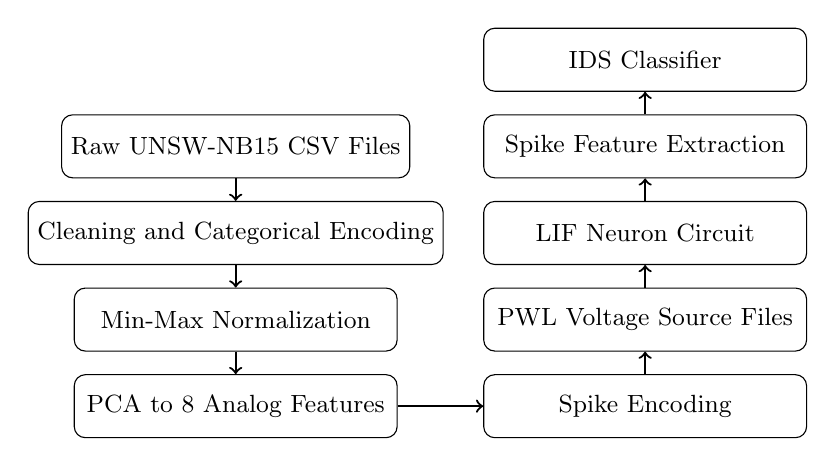
\begin{tikzpicture}[node distance=1.1cm, every node/.style={font=\small}]
\node[draw, rounded corners, minimum width=4.1cm, minimum height=0.8cm] (raw) {Raw UNSW-NB15 CSV Files};
\node[draw, rounded corners, below of=raw, minimum width=4.1cm, minimum height=0.8cm] (clean) {Cleaning and Categorical Encoding};
\node[draw, rounded corners, below of=clean, minimum width=4.1cm, minimum height=0.8cm] (norm) {Min-Max Normalization};
\node[draw, rounded corners, below of=norm, minimum width=4.1cm, minimum height=0.8cm] (pca) {PCA to 8 Analog Features};
\node[draw, rounded corners, right of=pca, xshift=4.1cm, minimum width=4.1cm, minimum height=0.8cm] (enc) {Spike Encoding};
\node[draw, rounded corners, above of=enc, minimum width=4.1cm, minimum height=0.8cm] (pwl) {PWL Voltage Source Files};
\node[draw, rounded corners, above of=pwl, minimum width=4.1cm, minimum height=0.8cm] (lif) {LIF Neuron Circuit};
\node[draw, rounded corners, above of=lif, minimum width=4.1cm, minimum height=0.8cm] (features) {Spike Feature Extraction};
\node[draw, rounded corners, above of=features, minimum width=4.1cm, minimum height=0.8cm] (cls) {IDS Classifier};
\draw[->, thick] (raw) -- (clean);
\draw[->, thick] (clean) -- (norm);
\draw[->, thick] (norm) -- (pca);
\draw[->, thick] (pca) -- (enc);
\draw[->, thick] (enc) -- (pwl);
\draw[->, thick] (pwl) -- (lif);
\draw[->, thick] (lif) -- (features);
\draw[->, thick] (features) -- (cls);
\end{tikzpicture}
\caption{Detailed architecture of the proposed neuromorphic IDS pipeline}
\label{fig:architecture}
\end{figure}

Figure \ref{fig:architecture} shows the full architecture. The left side represents dataset processing. The right side represents spike-domain and hardware-domain processing. The PWL file is the connecting artifact between software and circuit simulation.

\section{Data Pipeline Methodology}

The data pipeline follows a fixed sequence:
\begin{enumerate}
\item Load all raw UNSW-NB15 CSV files.
\item Concatenate records into a single dataframe.
\item Generate derived features such as packet rate.
\item Remove IP addresses, timestamps and binary label fields.
\item Clean missing or placeholder values.
\item Encode categorical fields into numerical values.
\item Normalize all features using Min-Max scaling.
\item Apply PCA to reduce the feature count.
\item Normalize PCA outputs again to the 0 to 1 range.
\item Save the processed analog feature dataset.
\end{enumerate}

This methodology ensures that the final file contains only hardware-facing analog features and the corresponding attack category label.

\section{PCA-to-Neuron Mapping}

The number of PCA components is selected based on the target number of physical input neurons. A direct mapping is used:
\begin{equation}
N_{PCA} = N_{input\_neurons}
\end{equation}
For the current design, $N_{PCA}=8$. This means each network sample is represented by eight analog feature values:
\begin{equation}
S_i = [p_1, p_2, p_3, p_4, p_5, p_6, p_7, p_8]
\end{equation}
where each $p_i$ is normalized between 0 and 1. This vector becomes the input to the spike encoder.

\section{Spike Encoding Methodology}

For each normalized PCA value, the encoder generates spike trains. Population coding uses multiple receptive fields per input feature. If $M$ is the number of population neurons per feature, the total number of input spike channels is:
\begin{equation}
N_{channels} = N_{PCA} \times M
\end{equation}
With eight PCA features and four population neurons per feature:
\begin{equation}
N_{channels} = 8 \times 4 = 32
\end{equation}

\begin{table}[H]
\centering
\caption{Spike encoding design parameters}
\label{tab:encodingparams}
\begin{tabular}{|p{0.35\textwidth}|p{0.35\textwidth}|}
\hline
\textbf{Parameter} & \textbf{Selected value} \\
\hline
Number of PCA features & 8 \\
\hline
Population neurons per feature & 4 \\
\hline
Total PWL input channels per sample & 32 \\
\hline
Spike window length & 10 timesteps \\
\hline
Spike voltage low/high & 0 V / 1 V \\
\hline
\end{tabular}
\end{table}

\section{PWL File Interface}

The PWL file interface is the most important design decision for interdisciplinary integration. It allows the ISE-side software pipeline to produce a file that the ECE-side Cadence/LTSpice circuit can use directly. Each file contains a single spike train. The folder structure stores all PWL files for one sample together.

For example, a population-coded sample may contain files such as:
\begin{verbatim}
sample_0_cat_6/
  V_neuron_0_m_0.txt
  V_neuron_0_m_1.txt
  V_neuron_0_m_2.txt
  V_neuron_0_m_3.txt
  ...
\end{verbatim}

Here, \texttt{V\_neuron\_0} refers to the first PCA feature and \texttt{m\_1} refers to the second population receptive field for that feature.

\section{LIF Circuit Interface Design}

The LIF circuit block requires an input voltage waveform, a membrane node and an output node. The input voltage waveform is supplied by a PWL file. The membrane node should show the characteristic rise due to integration and fall due to leakage or reset. The output node should generate a pulse when the membrane voltage crosses the threshold.

\begin{table}[H]
\centering
\caption{Expected observable nodes for LIF circuit simulation}
\label{tab:lifnodes}
\begin{tabular}{|p{0.28\textwidth}|p{0.55\textwidth}|}
\hline
\textbf{Node} & \textbf{Purpose} \\
\hline
Input voltage & Verifies that the generated PWL file is applied correctly. \\
\hline
Membrane voltage & Shows integration, leakage and reset behaviour. \\
\hline
Output voltage & Indicates threshold crossing and generated spikes. \\
\hline
\end{tabular}
\end{table}

\section{Spike Feature Extraction Design}

After simulation, the output waveform can be converted into numerical features. A threshold-based rising-edge detector is used to avoid counting the same output pulse multiple times. If the output voltage crosses from low to high, one spike is counted. The extracted features may include:
\begin{enumerate}
\item Spike count.
\item First spike time.
\item Mean inter-spike interval.
\item Standard deviation of inter-spike interval.
\item Firing rate.
\item Maximum membrane voltage.
\end{enumerate}

These features form the bridge between the analog neuron response and the final IDS classifier.

\section{Validation Methodology}

The project validation is planned in layered stages:
\begin{enumerate}
\item Verify processed CSV generation from the raw dataset.
\item Verify that PCA output has the expected number of columns and bounded values.
\item Verify that spike trains match the selected encoding method.
\item Verify that generated PWL files contain valid time-voltage pairs.
\item Verify that a selected PWL file can drive a LIF neuron circuit.
\item Verify that membrane and output waveforms can be converted into spike features.
\end{enumerate}

This layered strategy reduces debugging difficulty. If the final classifier performs poorly, the team can inspect whether the issue comes from preprocessing, encoding, PWL generation, circuit behaviour or feature extraction.

\section{Risk and Design Mitigation}

Several risks are considered in the design. PCA may discard useful information if too few components are selected. To mitigate this, the number of components is aligned with hardware constraints while preserving as much variance as possible. PWL files may create sharp transitions that affect simulator convergence, so the encoder includes a small rise/fall duration. LIF circuits may be sensitive to threshold and leakage settings, so the design requires observable membrane and output nodes for calibration.

\section{Design Summary}

The design connects a real IDS dataset to a neuromorphic circuit interface. The main contribution of the design is not only the classifier workflow but the construction of a data-to-PWL path. This allows network traffic features to become voltage waveforms that can stimulate LIF neuron circuits. The next chapter explains how this design is implemented in the deployed system.

